\documentclass[]{article}
\usepackage{lmodern}
\usepackage{amssymb,amsmath}
\usepackage{ifxetex,ifluatex}
\usepackage{fixltx2e} % provides \textsubscript
\ifnum 0\ifxetex 1\fi\ifluatex 1\fi=0 % if pdftex
  \usepackage[T1]{fontenc}
  \usepackage[utf8]{inputenc}
\else % if luatex or xelatex
  \ifxetex
    \usepackage{mathspec}
  \else
    \usepackage{fontspec}
  \fi
  \defaultfontfeatures{Ligatures=TeX,Scale=MatchLowercase}
\fi
% use upquote if available, for straight quotes in verbatim environments
\IfFileExists{upquote.sty}{\usepackage{upquote}}{}
% use microtype if available
\IfFileExists{microtype.sty}{%
\usepackage{microtype}
\UseMicrotypeSet[protrusion]{basicmath} % disable protrusion for tt fonts
}{}
\usepackage[margin=1in]{geometry}
\usepackage{hyperref}
\hypersetup{unicode=true,
            pdfborder={0 0 0},
            breaklinks=true}
\urlstyle{same}  % don't use monospace font for urls
\usepackage{graphicx,grffile}
\makeatletter
\def\maxwidth{\ifdim\Gin@nat@width>\linewidth\linewidth\else\Gin@nat@width\fi}
\def\maxheight{\ifdim\Gin@nat@height>\textheight\textheight\else\Gin@nat@height\fi}
\makeatother
% Scale images if necessary, so that they will not overflow the page
% margins by default, and it is still possible to overwrite the defaults
% using explicit options in \includegraphics[width, height, ...]{}
\setkeys{Gin}{width=\maxwidth,height=\maxheight,keepaspectratio}
\IfFileExists{parskip.sty}{%
\usepackage{parskip}
}{% else
\setlength{\parindent}{0pt}
\setlength{\parskip}{6pt plus 2pt minus 1pt}
}
\setlength{\emergencystretch}{3em}  % prevent overfull lines
\providecommand{\tightlist}{%
  \setlength{\itemsep}{0pt}\setlength{\parskip}{0pt}}
\setcounter{secnumdepth}{0}
% Redefines (sub)paragraphs to behave more like sections
\ifx\paragraph\undefined\else
\let\oldparagraph\paragraph
\renewcommand{\paragraph}[1]{\oldparagraph{#1}\mbox{}}
\fi
\ifx\subparagraph\undefined\else
\let\oldsubparagraph\subparagraph
\renewcommand{\subparagraph}[1]{\oldsubparagraph{#1}\mbox{}}
\fi

%%% Use protect on footnotes to avoid problems with footnotes in titles
\let\rmarkdownfootnote\footnote%
\def\footnote{\protect\rmarkdownfootnote}

%%% Change title format to be more compact
\usepackage{titling}

% Create subtitle command for use in maketitle
\newcommand{\subtitle}[1]{
  \posttitle{
    \begin{center}\large#1\end{center}
    }
}

\setlength{\droptitle}{-2em}

  \title{}
    \pretitle{\vspace{\droptitle}}
  \posttitle{}
    \author{}
    \preauthor{}\postauthor{}
    \date{}
    \predate{}\postdate{}
  

\begin{document}

\section{Présentation de
l'entreprise}\label{presentation-de-lentreprise}

Mon stage de fin d'études, se déroule dans à l'université de l'UMons
dans le service d'Écologie Numérique des Milieux Aquatiques (abrégé en
EcoNum) du département de Biologie.

L'Université de Mons (UMONS), est une université francophone implantée
en Belgique, dans la province du Hainaut. Elle est constituée de 2
Ecoles et de 7 Facultés, dont la faculté des Sciences.

Le Département de biologie de la faculté des Sciences est impliqué dans
la formation des étudiants et dans la recherche.

Le service d'Écologie Numérique des Milieux Aquatiques travaille dans
l'enseignement des biostatistiques et de l'écologie aquatique à
l'Université de Mons.

Le laboratoire EcoNum étudie les systèmes biologiques aquatiques
complexes, tels les communautés planctoniques et les récifs coralliens,
face aux changements de leur environnement.

Le laboratoire développe aussi des outils de traitement statistique, y
compris dans le domaine du data mining, des big data, et de la recherche
reproductible. Il participe à des études sur les logiciels Open Source
et développe des chémostats.

Le laboratoire d'EcoNum est situé sur le campus de la plaine de Nimy (A)
(voir figure 1.1) dans le pentagone (1) (voir figure 1.2).

\begin{figure}
\centering
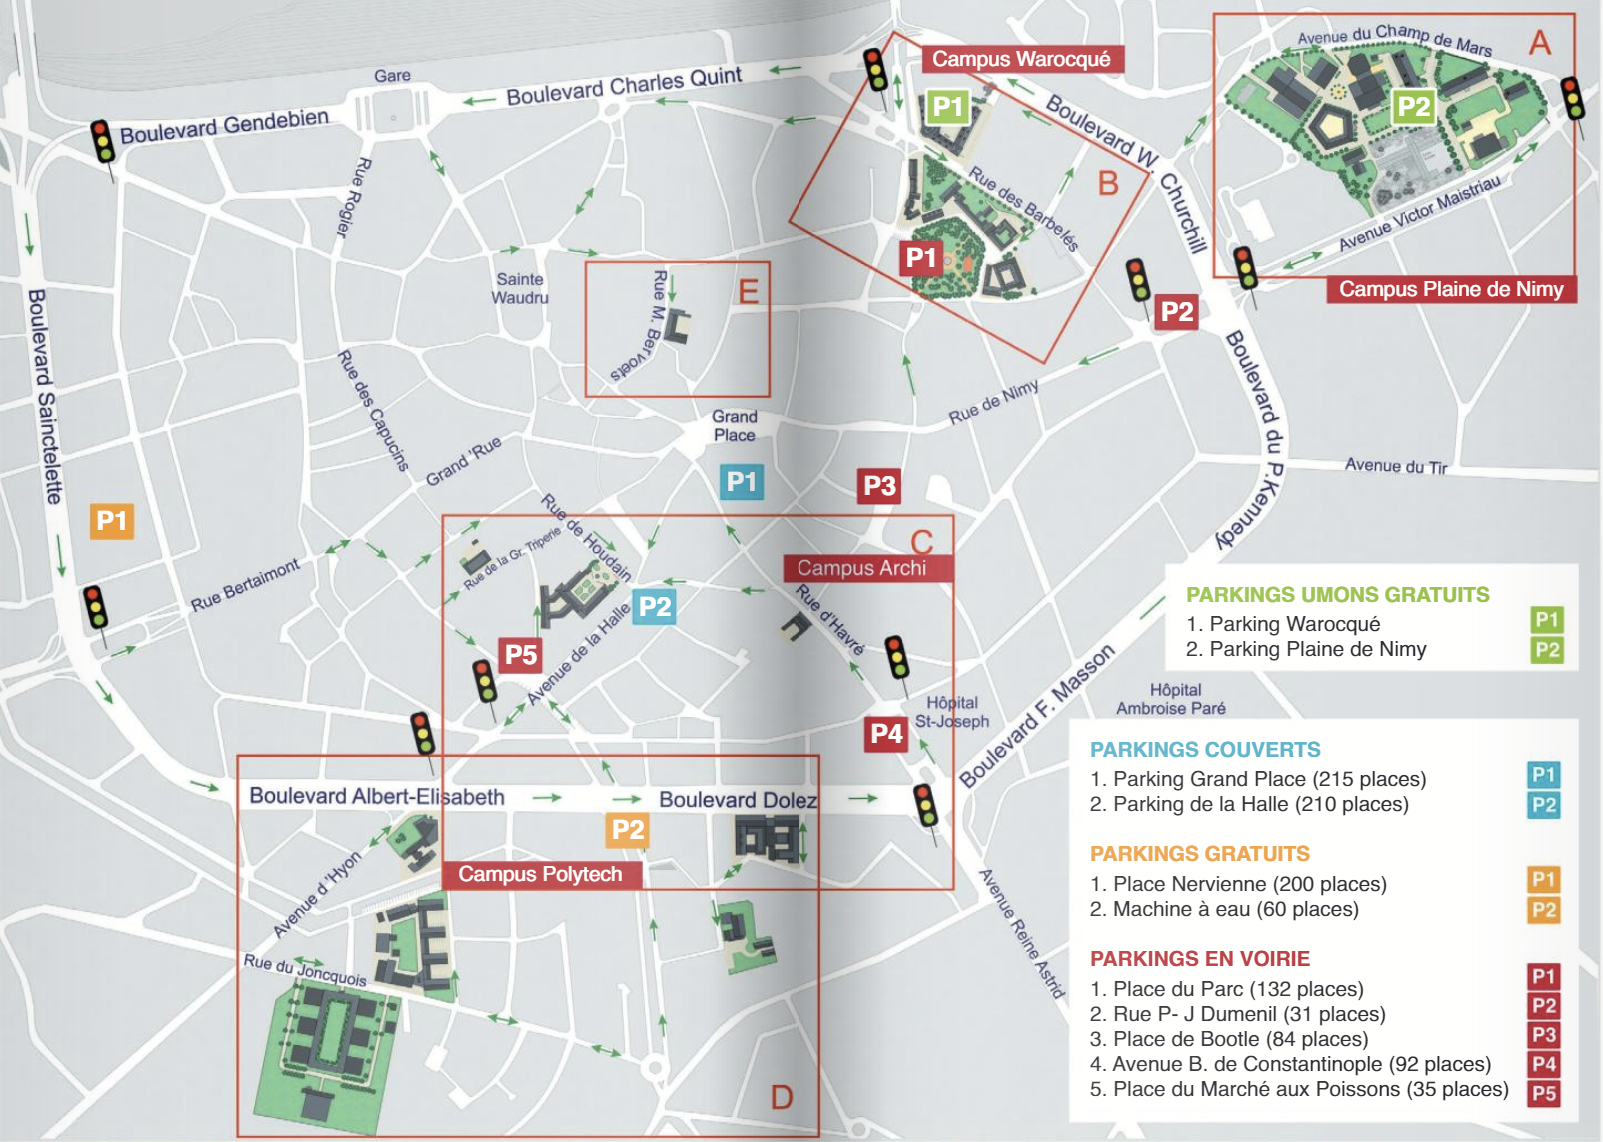
\includegraphics{../image/plan-campus.png}
\caption{Carte de la ville de Mons}
\end{figure}

\begin{figure}
\centering
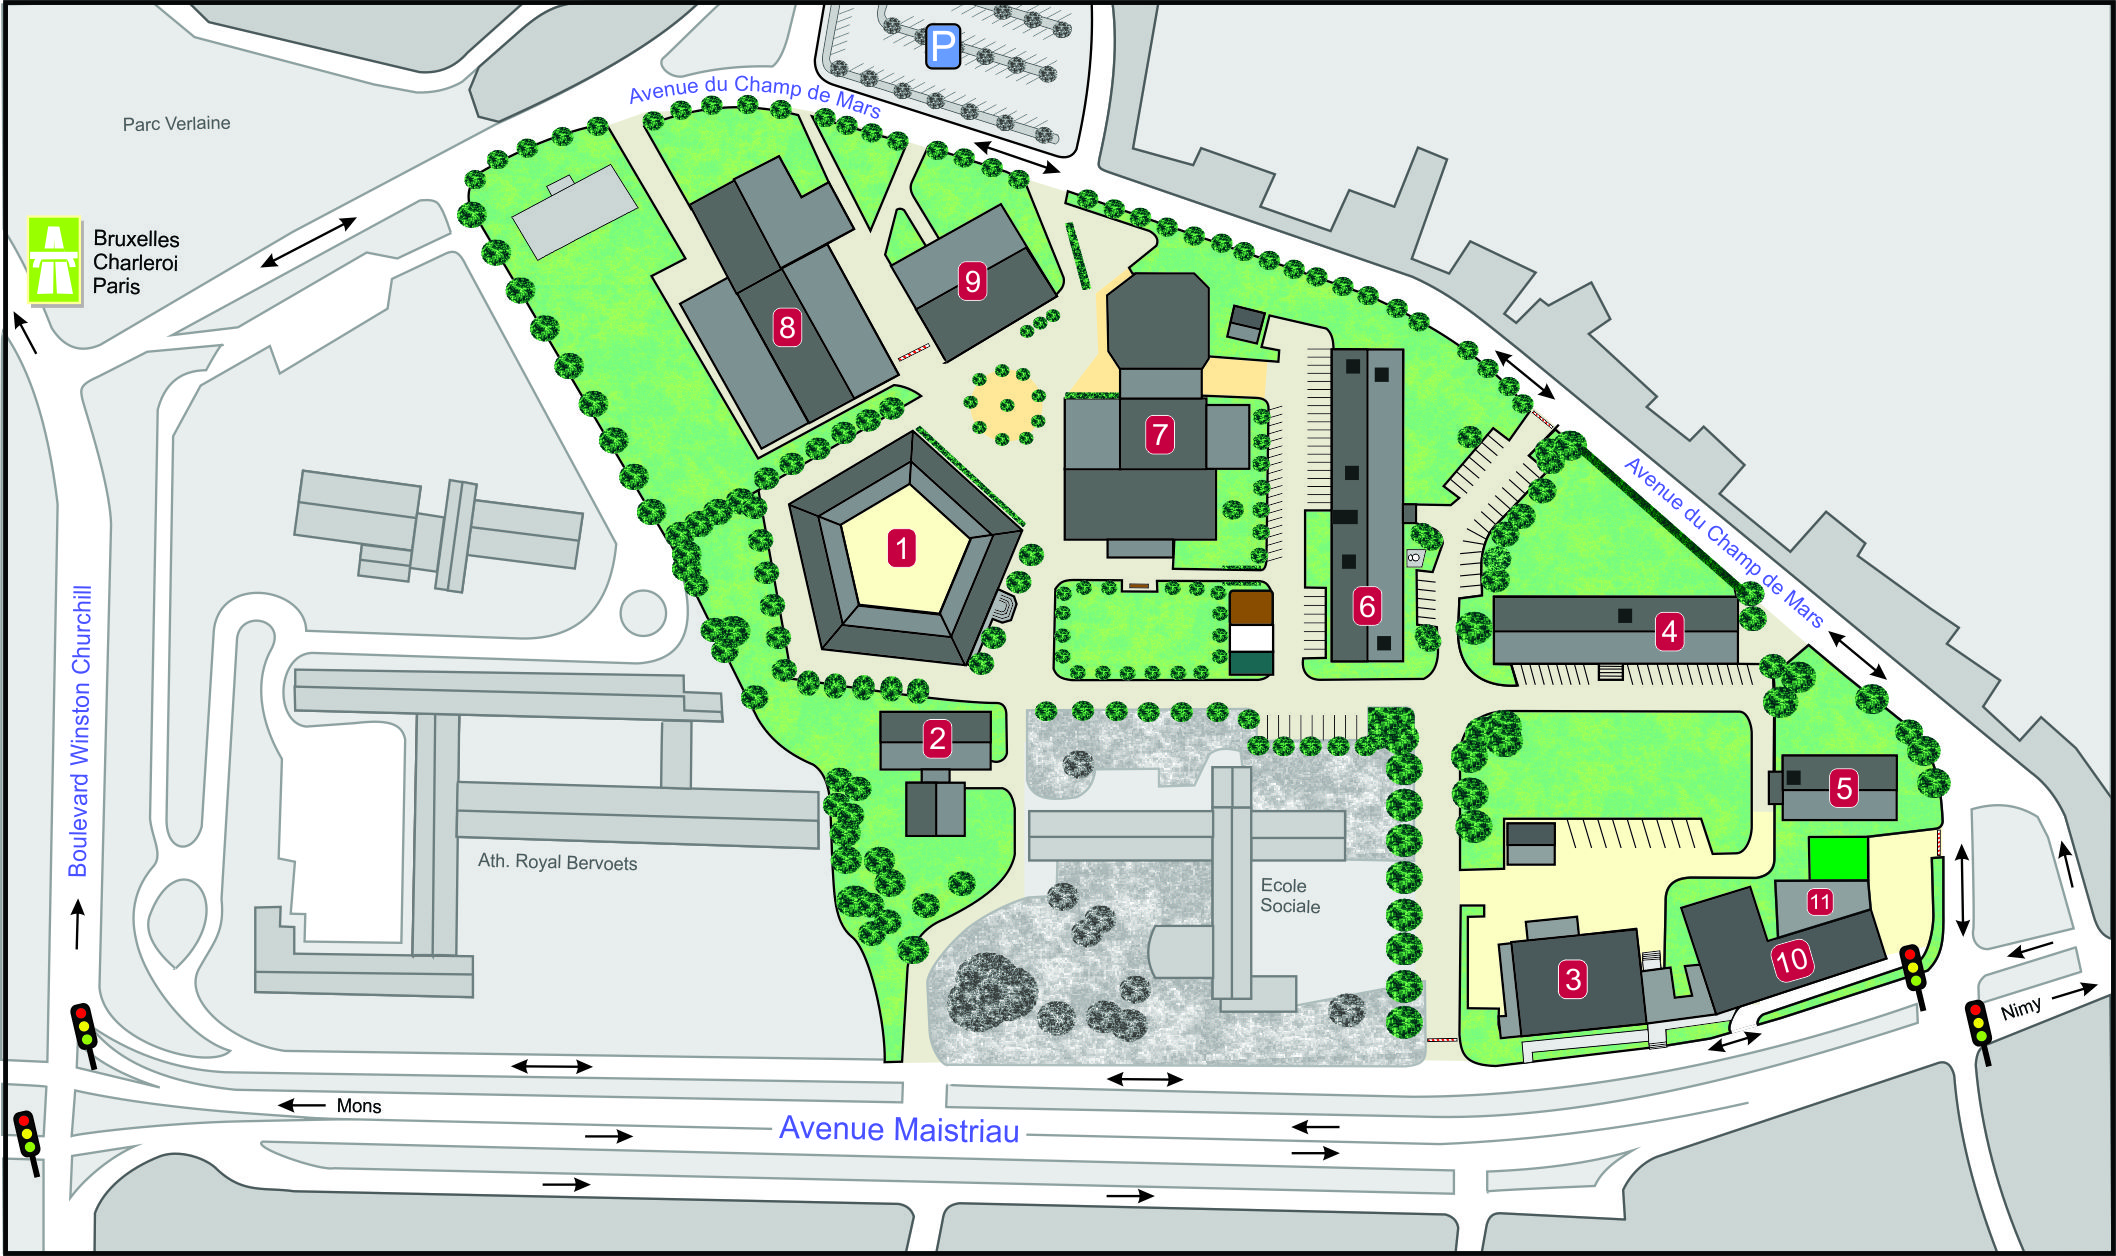
\includegraphics{../image/plaine-Nimy.jpg}
\caption{Carte du campus de la plaine de Nimy}
\end{figure}

\section{Présentation de l'équipe}\label{presentation-de-lequipe}

\subsection{Philippe Grosjean}\label{philippe-grosjean}

\begin{figure}[h!]
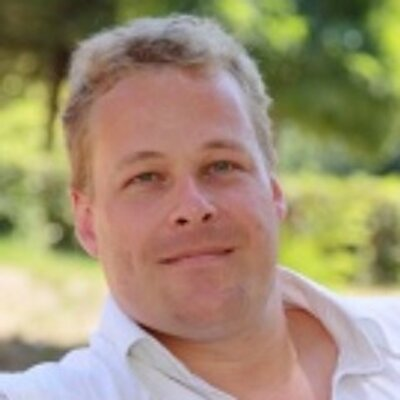
\includegraphics[width=4cm]{../image/Grosjean2.jpg}
\caption{Monsieur Philippe Grosjean, chef du service d'EcoNum.}
\end{figure}

Mon maître de stage est Monsieur Philippe Grosjean, il enseigne les
biostatistiques, l'écologie aquatique, l'écophysiologie et
l'océanographie générale aux étudiants biologistes.

Il travaille également dans le domaine de la recherche sur plusieurs
projets, dont l'identification automatique du plancton par photographie,
des algorithmes de \emph{machine learning}, développement de logiciel
pour l'écologie.

Il développe des outils Open Source comme la \emph{SciViews Box}, qui
est une machine virtuelle contenant une suite de logiciel pré-configuré
pour l'utilisation de ses étudiants.

Il encadre 1 doctorant et 2 étudiants en masters.

\subsection{Guyliann Engels}\label{guyliann-engels}

\begin{figure}[H]

\includegraphics[width=4cm]{../image/Guyliann.jpg}
\caption{Guyliann Engels, doctorant encadrant le stage.}
\end{figure}

Guyliann Engels est chercheur et professeur-assistant, il effectue sa
thèse sur l'écophysiologie du corail, où il utilise un mésocosme pour
étudier les stress des coraux engendrés par la modification de leurs
nutriments essentiels. Il utilise fréquemment les outils de statistiques
R et RStudio (avec R Markdown, R Notebook).

Il encadre mon travail.

\subsection{Antoine Batigny}\label{antoine-batigny}

\begin{figure}[h!]
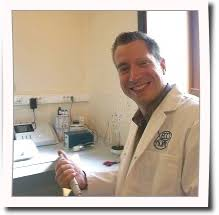
\includegraphics[width=4cm]{../image/antoine2.jpg}
\caption{Technicien du service d'EcoNum.}
\end{figure}

Antoine Batigny est technicien, c'est lui qui s'occupe de gérer les
mésocosmes et de l'auto-analyseur.

\subsection{Rémy Dugauquier}\label{remy-dugauquier}

\begin{figure}[h!]
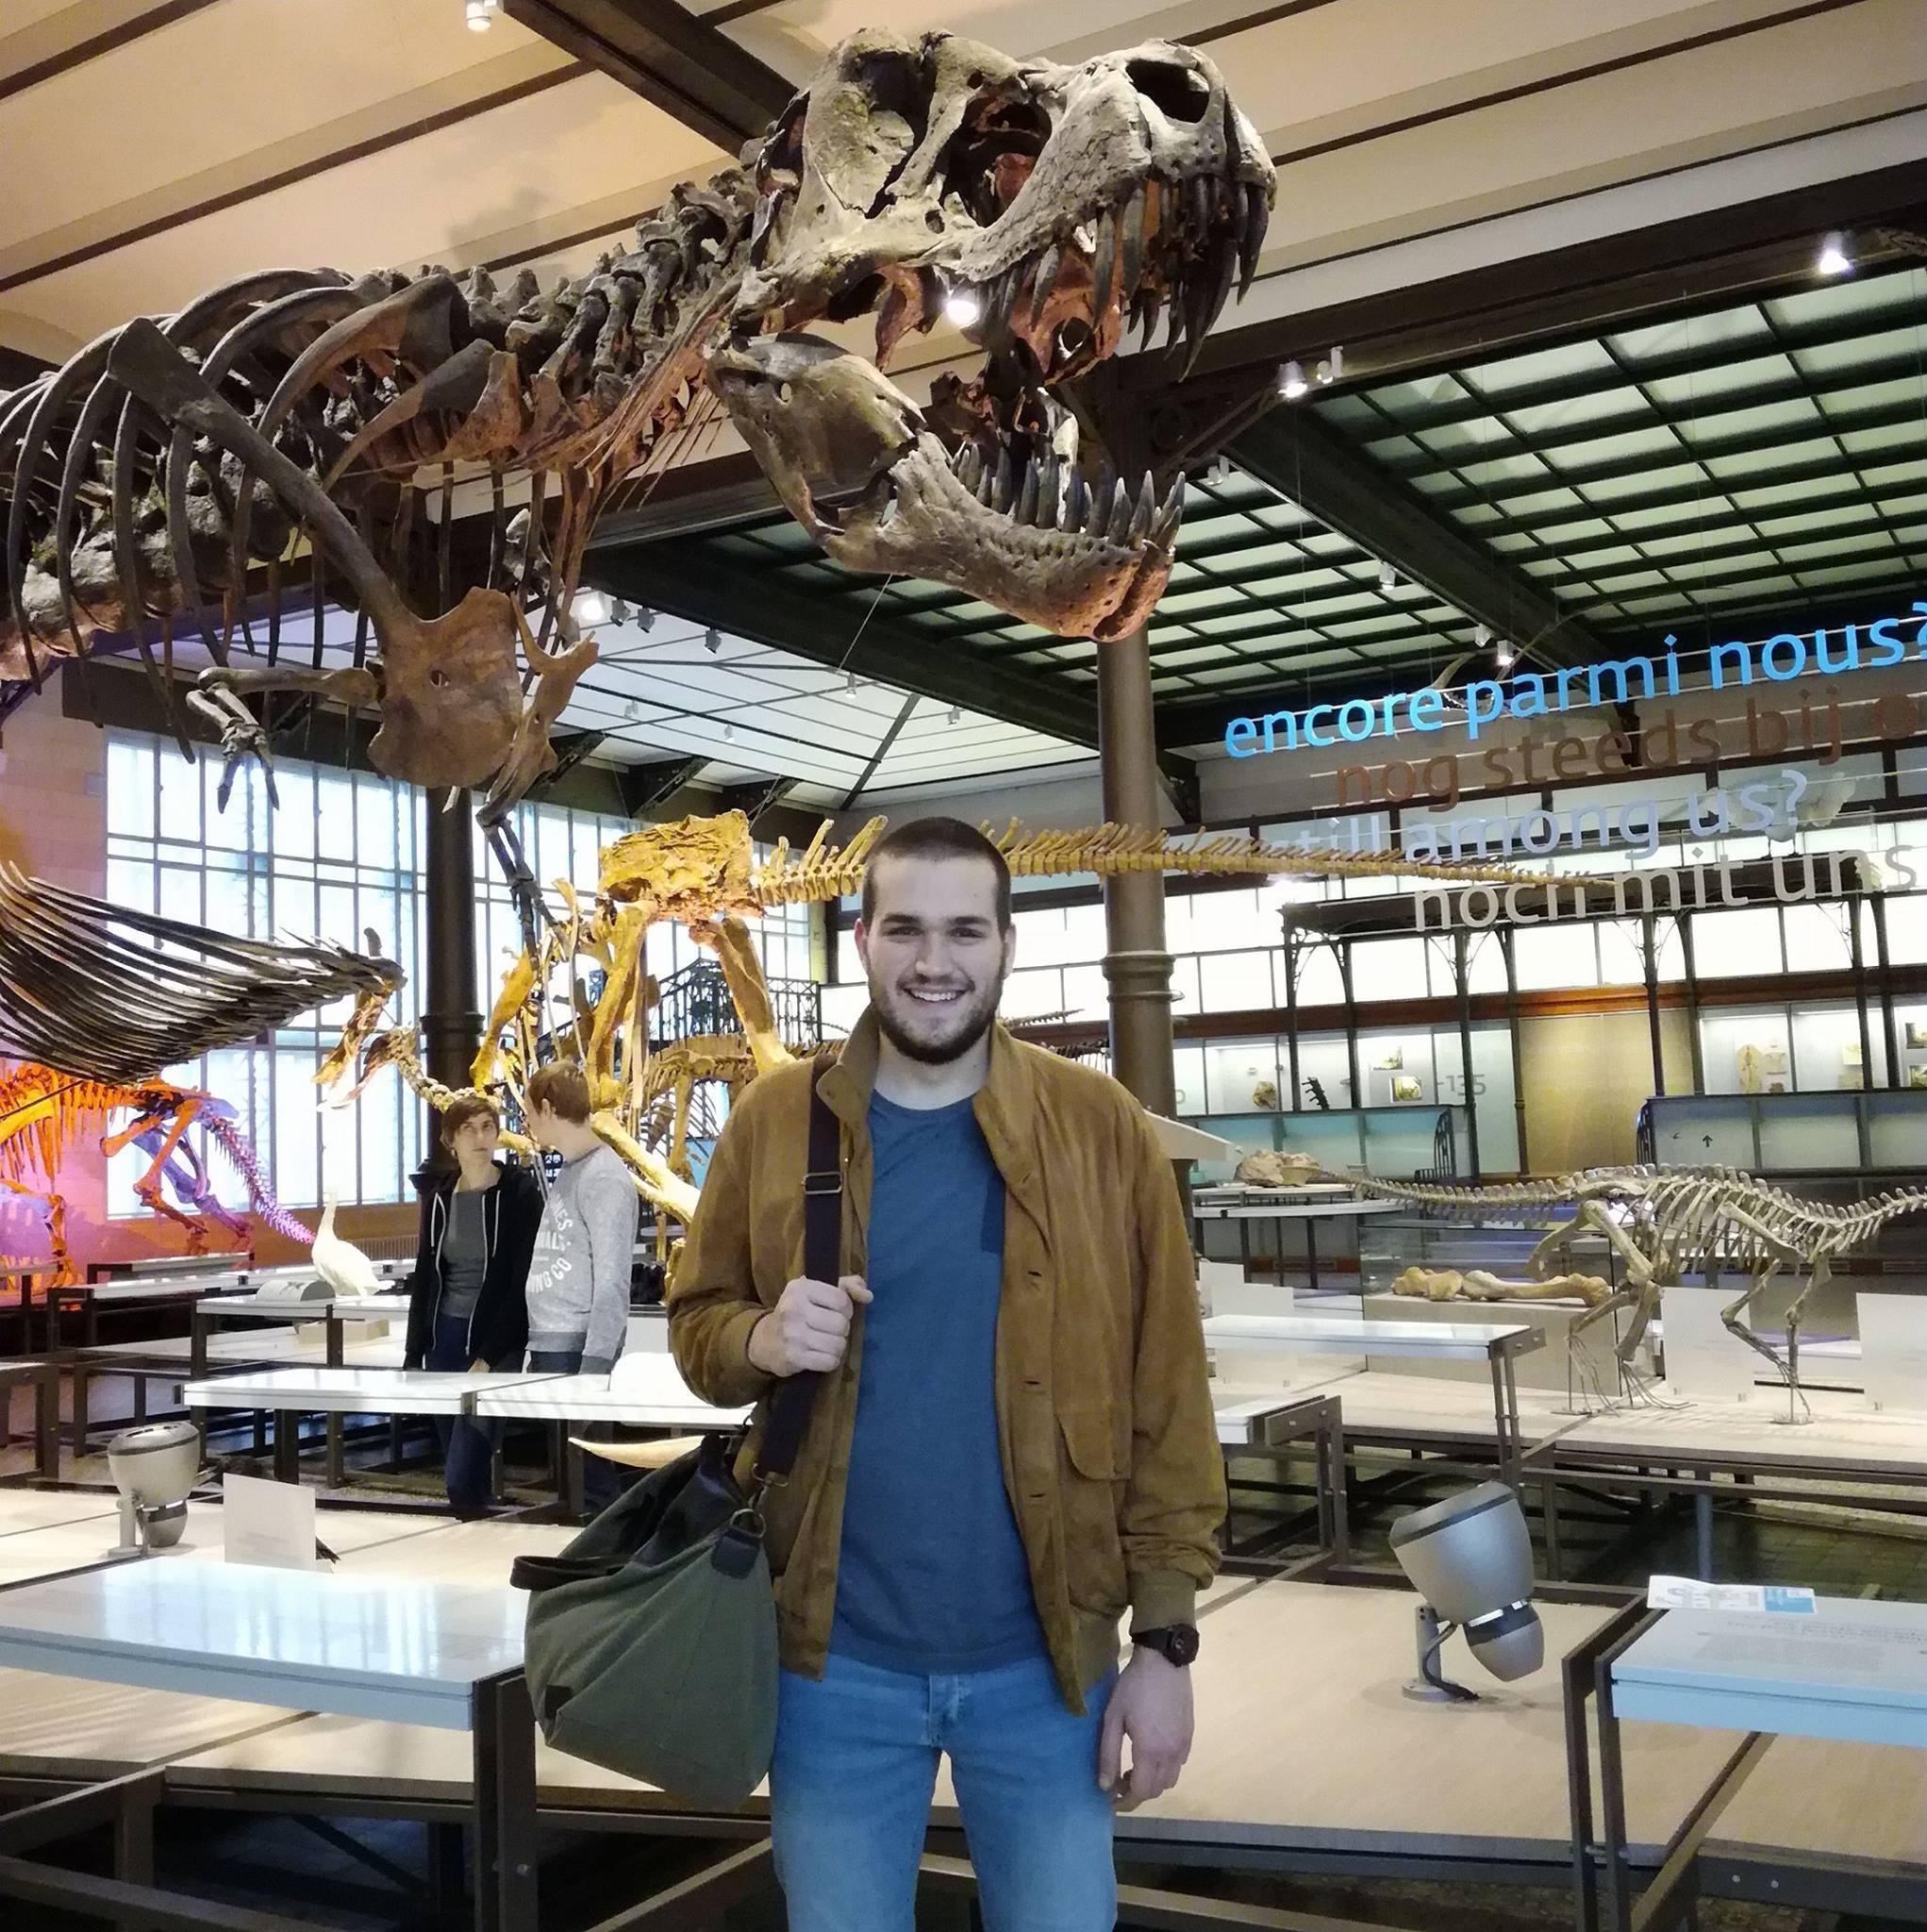
\includegraphics[width=4cm]{../image/remy.jpg}
\caption{Etudiant en master}
\end{figure}

Rémy Dugauquier est en dernière année de master et fait son TFE sur le
plancton. \textbf{à développer}

\subsection{Madeleine Gille}\label{madeleine-gille}

\begin{figure}[h!]
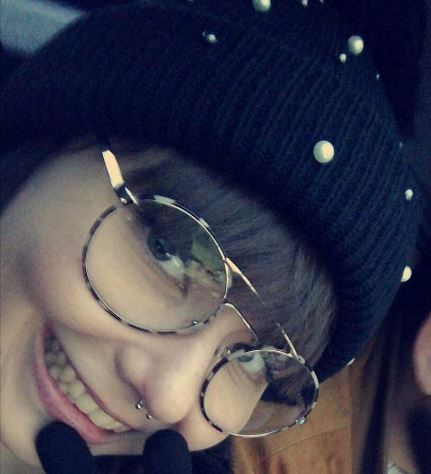
\includegraphics[width=4cm]{../image/madeleine.jpg}
\caption{Etudiante en master}
\end{figure}

Madeleine Gille est en dernière année de master et fait son TFE sur le
corail. \textbf{à développer}


\end{document}
